\documentclass{standalone}
\usepackage{tikz}
\usepackage{ctex,siunitx}
\usepackage{tkz-euclide}
\usepackage{amsmath}
\usetikzlibrary{patterns, calc}
\usetikzlibrary {decorations.pathmorphing, decorations.pathreplacing, decorations.shapes,}
\begin{document}
\small
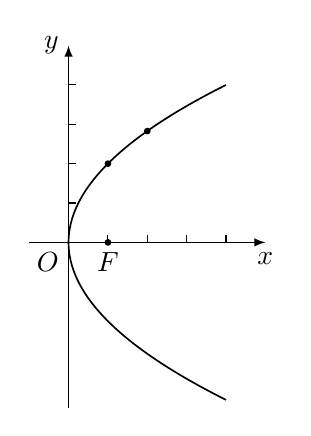
\begin{tikzpicture}[>=latex,scale=0.5]
  \draw[thin,->](-1,0)--(5,0)node[below]{$x$};
  \draw[thin,->](0,-4.2)--(0,5)node[left]{$y$};
  \tkzDefPoints{0/0/O,1/2/A,2/2.828/B,1/0/F}
  \foreach \x in {1,...,4} 
    {
      \draw[thin,densely dashed] (\x,0)--(\x,0.2);
      \draw[thin,densely dashed] (0,\x)--(0.2,\x);
    }
  \draw[semithick,samples=200,domain=-4:4] plot ({0.25*\x*\x},{\x});
  \tkzDrawPoints[fill=black](A,B,F)
  \tkzLabelPoints[below left](O)
  \tkzLabelPoints[below](F)
\end{tikzpicture}
\end{document}